\chapter{La création des objets}

\section{Reconnaissance vocale : Application Android}
	\subsection{Etat de l’art}	
Tout projet implique une phase de recherche, afin d'effectuer un état de l'art sur ce qu'il a déjà été fait 
auparavant dans ce domaine. Afin de rechercher ce qu'il fallait pour cet état de l'art, il a donc fallu 
décomposer en plusieurs parties ce que devait réellement réaliser cette reconnaissance. Ces parties étaient :

\begin{itemize}
\item Activation de la reconnaissance vocale automatiquement
\item Gestion de la chaîne de caractères comprise par la reconnaissance
\end{itemize}

De base sur Android, il est possible d'activer la reconnaissance vocale  automatiquement grâce aux mots clefs 
« OK Google ». Souhaitant appeler notre intelligence domotique Jarvis, il était peu souhaitable de dire ces 
mots afin d'activer la reconnaissance.
Après recherches, il s'avère qu'il n'existe aucun moyen simple de changer ces mots clefs, puisque les seuls 
moyens sont soit d'avoir un téléphone rooté, autrement dit où l'on a tous les accès afin de changer le bon 
fichier de configuration. Soit d'avoir un téléphone de la marque Motorola, qui intègre le changement de ces 
mots directement dans son firmware. C'est pourquoi pour activer la reconnaissance vocale, nous sommes obligés 
de prononcer les mots « OK Google ».
	
	\subsection{Activation de la reconnaissance vocale}
	
Afin de pouvoir démarrer et utiliser la reconnaissance vocale, il faut un ensemble d'éléments :
\begin{itemize}
 \item Autovoice
 \item Tasker
\end{itemize}

\begin{figure}[!ht]
         \centering
         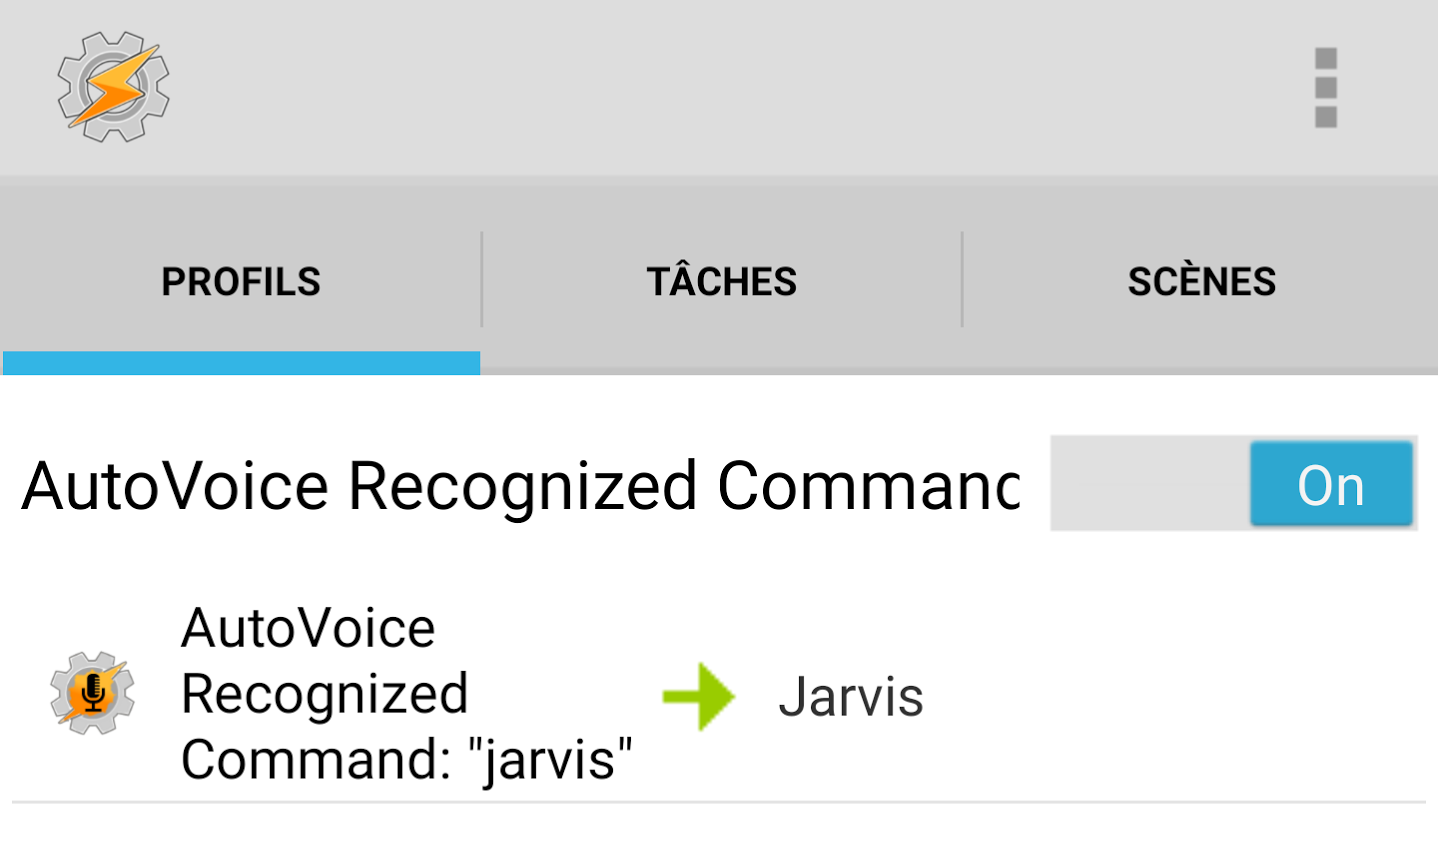
\includegraphics[width=0.5\textwidth]{img/tasker.png}
         \caption{Autovoice + Tasker}
         \label{Tasker}
\end{figure}

Autovoice est une application Android qui permet d'utiliser la reconnaissance vocale de Google, et de se 
servir de la chaîne de caractères reconnues pour en faire ce que l'on souhaite. Par ailleurs, on peut la 
paramétrer de telle sorte qu'elle réagisse seulement si une suite de mots clefs est reconnue, comme sur la 
figure \ref{Tasker}. Afin de pouvoir communiquer avec Jarvis, le seul mot clef choisi a donc été son nom. Du 
côté de Tasker, c'est une application d'automatisation très connue sur Android. Elle permet de réaliser des 
tâches en réponse à un événement donné. Ainsi il est possible d'utiliser comme événement Autovoice, et comme 
tâche, une application qui permet de traiter la chaîne de caractères : SpeechToText, comme on peut le voir 
sur la figure \ref{jarvis}.

\begin{figure}[!ht]
         \centering
         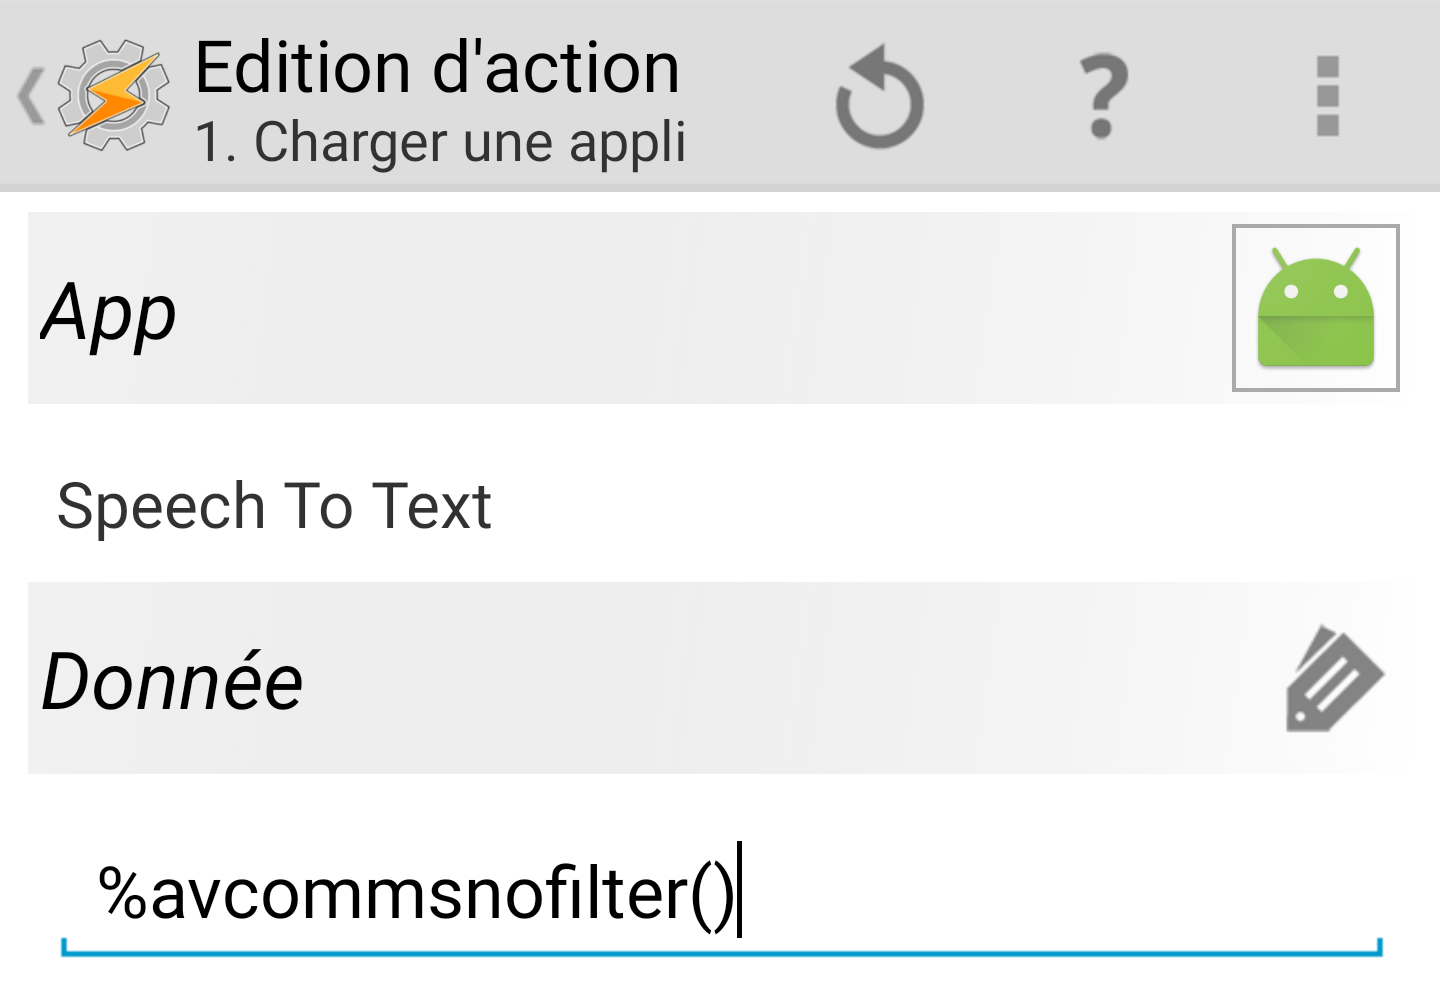
\includegraphics[width=0.5\textwidth]{img/jarvis.png}
         \caption{Tâche jarvis}
         \label{jarvis}
\end{figure}

	\subsection{SpeechToText}
	
	  \subsubsection{La base de données}
	
SpeechToText est une application Android qui permet donc d'interpréter une chaîne de caractères, et 
d'envoyer une trame suivant le protocole SDCP au bon objet connecté. l'application possède deux bases de 
données dynamiques. La première possède l'ensemble des objets intelligents. Cette base de données est stockée 
dans un 
fichier JSON.

\begin{figure}[!ht]
         \centering
         	\begin{lstlisting}
{
    "smartDevices" : [
      {
	"device": {
	  "idAction": "0x111",
	  "bleName": "sdc_Lisa"
	}
      }]
}
		\end{lstlisting}
         \caption{Base de données des objets intelligents}
         \label{BDD_smart}
\end{figure}


Cette base de données comprend une liste des objets connectés proches de nous. Comme on peut le voir un objet 
est caractérisé par deux choses : l'identifiant de l'action qu'il peut réaliser, ainsi que le nom de l'objet 
bluetooth auquel il faut se connecter pour réaliser l'action.

\begin{figure}[!ht]
         \centering
	 \begin{lstlisting}[caption=][frame=single]
{
    "voiceCommands" : [
      {
        "command" : {
            "voiceActivation" : "Quelle est la température",
            "voiceDiction" : "la température est",
            "idAction" : "0x111"
        }
      }]
}
	 \end{lstlisting}
         \caption{Base de données des commandes vocales}
         \label{BDD_objects}
\end{figure}



Ainsi une commande vocale est caractérisée par une chaîne de caractères à reconnaître, une chaîne de 
caractères à dire par synthèse vocale, afin de donner un feedback sur ce qu'il se passe à l'utilisateur. Elle 
contient elle aussi l'identifiant de l'action à réaliser, afin de faire le lien avec l'autre base de données.

La première chose à faire après avoir reçue la phrase reconnue par la reconnaissance vocale, est de 
reconnaître quelle requête l'utilisateur souhaite réaliser. Pour ce faire, l'application réalise un algorithme 
sur la chaîne reçue, dont le but est d'évaluer la similarité avec l'ensemble des 
phrases possibles. La distance minimale caractérisera la requête faite par l'utilisateur. Il existe 
différents algorithmes, tel que: Levenshtein, ou JaroWinkler.

    \subsubsection{La distance de Levenshtein}
C'est le plus simple des deux algorithmes. Cette distance calcule le nombre de différences 
qu'il y a entre deux chaînes de caractères. Ces différences peuvent être le remplacement, la suppression, 
ou l'insertion d'un caractère.

    \subsubsection{La distance de JaroWinkler} 
Celle-ci part de la distance de Jaro dont l'équation est [1]: 
\begin{equation}
 d = \frac{1}{3}(\frac{m}{|s1|}+\frac{m}{|s2|}+\frac{m-t}{m})
\end{equation}

où :
\begin{itemize}
 \item $|s_i|$ est la longueur de la chaîne de caractères de la chaîne 'i'
 \item $m$ est le nombre de caractères \emph{correspondants} dans les 2 chaînes
 \item $t$ est le nombre de \emph{transpositions} nécessaires de ces caractères partagés
\end{itemize}

Deux caractères identiques de $s_1$ et $s_2$ sont dit \emph{correspondants} lorsque leur éloignement dans 
leur chaîne respective ne dépasse pas :
\begin{equation}
 \lfloor{\frac{max(|s_1|, |s_2|)}{2}}\rfloor - 1
\end{equation}

Le nombre de \emph{transpositions} est obtenu en comparant le i-ème caractère \emph{correspondant} de $s_1$ 
avec le i-ème caractère \emph{correspondant} de $s_2$. Le nombre de fois où ces caractères sont différents, 
divisé par deux, donne le nombre de transpositions.

puis on calcule la distance avec cette équation :
\begin{equation}
 d_w = d_j + (l_p(1-d_j))
\end{equation}

avec :
\begin{itemize}
 \item $d_j$, la distance de Jaro entre $s_1$ et $s_2$
 \item $l$, la longueur du préfixe commun (avec un maximum de 4 caractères)
 \item $p$, un coefficient qui permet de favoriser les chaînes avec un préfixe commun. Winkler propose 
pour valeur $p=0.1$.

\end{itemize}

Wikipédia donne un très bon exemple pour comprendre cette distance. Ils appliquent cette algorithme pour 
calculer la distance entre MARTHA et MARHTA. Pour cela ils dressent un tableau :

\begin{figure}[!ht]
         \centering
	    \begin{tabular}{|0|1|2|3|4|5|6|}
		\hline
		& M & A & R & T & H & A \\
		\hline
		M & 1 & 0 & 0 & 0 & 0 & 0 \\
		\hline
		A & 0 & 1 & 0 & 0 & 0 & 0 \\
		\hline
		R & 0 & 0 & 1 & 0 & 0 & 0 \\
		\hline
		H & 0 & 0 & 0 & 0 & \textbf{1} & 0 \\
		\hline
		T & 0 & 0 & 0 & \textbf{1} & 0 & 0 \\
		\hline
		A & 0 & 0 & 0 & 0 & 0 & 1 \\
		\hline
	      \end{tabular}
         \caption{Exemple pour la distance de JaroWinkler}
         \label{JaroWinkler}
\end{figure}

On a :
\begin{itemize}
  \item $m = 6$ (Nombre de 1 dans la matrice)
  \item $|s_1| = 6$ 
  \item $|s_2| = 6$
  \item Les caractères correspondants sont \{{M,A,R,T,H,A\} pour $s_{1}$ et \{{M,A,R,H,T,A\} pour $s_{2}$. 
\end{itemize}

On a donc 2 couples (T/H et H/T) de caractères \emph{correspondants} différents, soit deux 
demi-transpositions. D'où $t=\frac {2}{2}=1$.

La distance de Jaro est :

\begin{equation}
 d_j = \frac {1}{3}\left(\frac {6}{6}+ \frac {6}{6}+\frac {6-1}{6}\right)=0.944
\end{equation}

La distance de Jaro-Winkler avec $p=0.1$ avec un préfixe de longueur $\ell =3$ devient

\begin{equation}
  d_w=0.944+(3*0.1(1-0.944))=0.961
\end{equation}

\subsubsection{Etude de l'algorithme le plus approprié}
La meilleure distance pour notre projet a été trouvée en faisant une série de tests, en utilisant à chaque 
fois les deux algorithmes. Le test consiste à prendre plusieurs phrases présentes dans le fichier des 
commandes vocales, et à les dire un grand nombres de fois, avec différents tons de voix, différentes 
articulations, et différents volumes. Ensuite, pour chaque requête, une liste des différentes phrases 
comprises par la reconnaissance vocale est établie. Les deux algorithmes sont alors appliqués, pour voir 
lequel est le plus robuste, et nous donne la correspondance la plus grande entre la requête souhaitée, et les 
commandes comprises. Il s'avère que l'algorithme le plus simple  était le plus robuste pour notre étude, 
c'est donc la la distance de Levenshtein qui a été gardée. 

Maintenant que nous sommes capables de savoir quelle requête l'utilisateur souhaite envoyer, et à quel objet, 
il faut savoir comment l'envoyer.

	\subsection{Intégration du protocole avec JNI}
Le protocole a été construit pour être sur systèmes embarqués, avec le langage C++. Or l'objet reconnaissance 
vocale doit lui aussi l'utiliser afin de pouvoir communiquer convenablement avec les autres objets. Ainsi deux 
choix étaient possibles :
\begin{itemize}
 \item Réécrire le protocole sous Android
 \item Intégrer le protocole en réalisant une interface pour Android
\end{itemize}

C'est la deuxième option qui a été choisie, celant évitant de refaire une grosse partie du travail déjà 
réalisée.

Il faut savoir que le système Android fonctionne grâce à une machine virtuelle Java : \emph{Art} (Pour 
Android Run Time). Cette machine n'exécute de base à priori que du byte code Java, et non de l'assembleur que 
l'on pourrait obtenir en compilant un langage natif comme le C++. Grâce à \emph{JNI}, pour Java Native 
Interface, il est possible d'interfacer du code java, avec du code natif. Pour cela il suffit de compiler le 
code natif pour en faire une librairie, qu'il suffira se charger dans le programme. Cette librairie 
contient un ensemble de fonctionnalités déjà compilé, et qui peut donc être utilisé directement dans le 
programme.

\subsubsection{Intégration de la librairie [2]}
La première chose à faire est de créer une classe dans le code Java, elle contiendra plusieurs directives 
importantes, comme le chargement de la librairie, mais aussi le prototype de la fonction \emph{fromCpp} qui 
sera défini dans le code natif, cela permettra de créer le lien entre les deux langages. Il faut ensuite 
demander au compilateur java de créer un fichier d'en-tête à partir de cette classe, qui sera utilisée dans 
notre librairie plus tard.

Il faut ensuite écrire le corps de la fonction \emph{fromCpp}, dans un autre fichier C++. Afin de faire le 
lien avec le code java, il faut inclure le fichier d'en-tête tout juste créer. Par la suite, nous devons 
compiler ce code en précisant que nous souhaitons obtenir une librairie et pas un fichier exécutable. Cela 
nous donnera un fichier \emph{.so} sous Linux, ou un fichier \emph{.dll} sous Windows. Ce fichier devra 
être placé à la racine du projet, afin que la machine virtuelle java puisse le trouver pendant l'exécution.

Dès lors il sera possible d'utiliser du code natif, et donc de pouvoir se servir du protocole afin 
de pouvoir communiquer avec les différents objets, et cela grâce au bluetooth d'Android.


	\subsection{Communiquer avec le protocole BLE}
	  \subsubsection{Fonctionnement du BLE}
L'application Android a donc pour but d'utiliser le protocole Bluetooth Low Energy, pour transmettre les 
paquets aux différents objets connectés. Afin de pouvoir se servir de ce bluetooth, il faut commencer par 
effectuer un scan, afin de voir tous les objets supportant ce protocole aux alentours. Une fonction de 
callback est appelée pour chaque appareil détectée. On peut ensuite se connecter à cet appareil, afin d'être 
appairé avec celui-ci.

Tous les appareils utilisant le protocole BLE utilisent le GATT (\emph{Generic Attribute Profile}), afin 
d'envoyer et de recevoir des données sur le réseau. Il faut donc obtenir cette interface pour pouvoir 
communiquer en BLE. Une fois l'interface GATT obtenue, il est possible de récupérer l'ensemble des 
caractéristiques. Les caractéristiques sont l'ensemble des valeurs que l'appareil possède que l'on peut lire 
ou écrire. Elles sont composées d'un UUID (\emph{Universally Unique Identifier}), d'une propriété qui permet 
d'avoir une description lisible de la caractéristique, et enfin d'une valeur. Par conséquent, si l'on souhaite 
obtenir la valeur de température d'un objet, il faut récupérer la caractéristique dont la propriété est 
"température", puis simplement récupérer sa valeur.

Cette procédure ne peut être simplifiée, il est donc obligatoire d'effectuer un scan pour voir l'ensemble des 
objets bluetooth dans les environs, même si nous les connaissons déjà. Il est donc impossible via le BLE 
d'android de se connecter directement à un appareil à partir de son adresse MAC bluetooth, ce qui est 
dommage, car nous devons donc passer par un scan pas forcément nécessaire, afin de communiquer avec un objet 
proche de nous.


\section{Les objets intelligents}

Maintenant que les différentes briques ont été posées, il est possible de créer les différents objets
intelligents.

\begin{figure}[!tbp]
  \centering
  \begin{minipage}[b]{0.49\textwidth}
    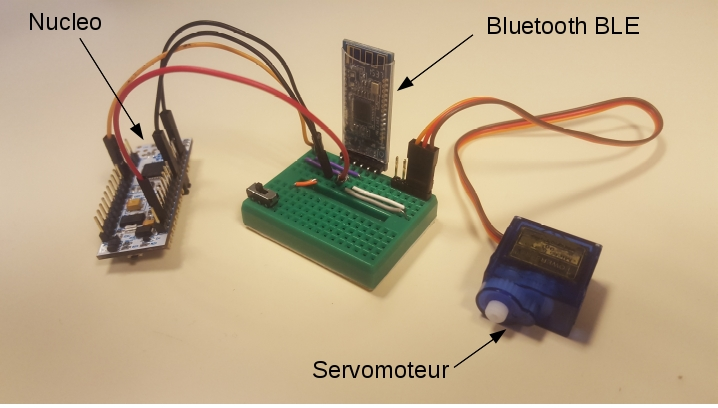
\includegraphics[width=0.95\textwidth]{img/actuator2.jpg}
    \caption{Actionneur intelligent}
    \label{actuator}
  \end{minipage}
  \hfill
  \begin{minipage}[b]{0.49\textwidth}
    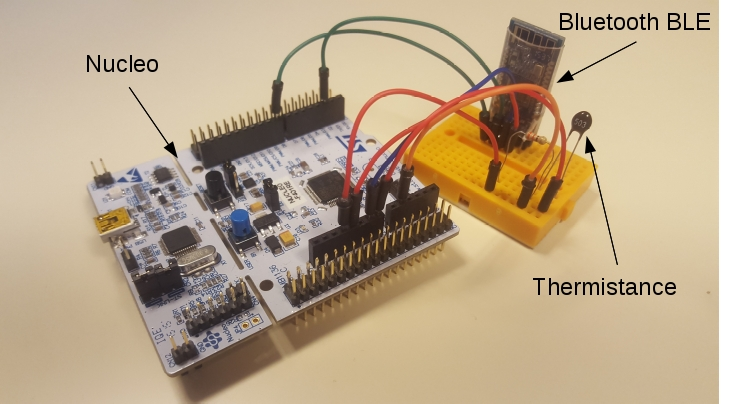
\includegraphics[width=0.95\textwidth]{img/sensor2.jpg}
    \caption{Capteur intelligent}
    \label{sensor}
  \end{minipage}
\end{figure}

Il est possible de voir sur les figures \ref{actuator} et \ref{sensor} que les deux objets ne possèdent pas la 
même carte de développement Nucleo. La carte présente pour l'actionneur est une F303K8, tandis que celle du 
capteur est une F401RE. De manière générale, la première possède moins de composants, mais est plus petite, 
qui est largement suffisant pour la création de nos objets connectés.

L'actionneur présent sur la figure \ref{actuator} est composé d'un servomoteur. Cet objet a été utilisé en 
tant qu'interrupteur intelligent. Le capteur présent sur la figure \ref{sensor} est quant à lui composé d'une 
thermistance, afin de pouvoir récupérer la température de la pièce.



